\documentclass[11pt]{article}

\linespread{1.0}

\newcommand{\bra}[1]{\left\langle #1 \right |}
\newcommand{\ket}[1]{\left | #1 \right\rangle}

\usepackage{mathtools}
\usepackage{floatrow}
\usepackage{bbold}
\usepackage{eurosym}
\usepackage{graphicx}
\usepackage{fullpage}
\usepackage{amsmath}
\usepackage{amsbsy}
\usepackage[all]{xy}
\usepackage[nottoc, notlof, notlot]{tocbibind}
\usepackage{makeidx}
\usepackage{multicol}
\usepackage{multirow}
\usepackage{float}
\usepackage{textcomp}
\usepackage[utf8]{inputenc}
\usepackage{bm}
\usepackage{appendix}
\usepackage{color}
\usepackage{listings}
\usepackage{slashed}
\usepackage{hyperref}
\usepackage{verbatim}
\usepackage{fancyhdr}
\usepackage{enumitem}
\usepackage[sans]{dsfont}
\usepackage{empheq}
\usepackage{feyn}
%\usepackage{noReferences}
\usepackage{booktabs}

\usepackage{array}
\newcolumntype{L}[1]{>{\raggedright\let\newline\\\arraybackslash\hspace{0pt}}m{#1}}
\newcolumntype{C}[1]{>{\centering\let\newline\\\arraybackslash\hspace{0pt}}m{#1}}
\newcolumntype{R}[1]{>{\raggedleft\let\newline\\\arraybackslash\hspace{0pt}}m{#1}}

\usepackage[headsep=0.8cm,headheight=0cm]{geometry}

\setlength{\oddsidemargin}{0.25in}
\setlength{\hoffset}{0.2in}
\setlength{\textwidth}{5.8in}
\setlength{\topmargin}{0.2in}
\setlength{\voffset}{-0.5in}
\setlength{\textheight}{8.8in}

\pagestyle{fancy}

\fancyhf{}
\lhead{LTD treatment of the quark self-energy}
%\rhead{Dr. Valentin Hirschi}
\rfoot{\thepage}


\definecolor{colKeys}{rgb}{0,0,1}
\definecolor{colIdentifier}{rgb}{0,0,0}
\definecolor{colCoxmments}{rgb}{0,0.5,1}
\definecolor{colString}{rgb}{0.6,0.1,0.1}

\lstset{%configuration de listings
float=hbp,%
basicstyle=\ttfamily\small, %
identifierstyle=\color{colIdentifier}, %
keywordstyle=\color{colKeys}, %
stringstyle=\color{colString}, %
commentstyle=\color{colComments}, %
columns=flexible, %
tabsize=2, %
frame=trBL, %
frameround=tttt, %
extendedchars=true, %
showspaces=false, %
showstringspaces=false, %
numbers=left, %
numberstyle=\tiny, %
breaklines=true, %
breakautoindent=true, %
captionpos=b,%
}

\date{\today}

\makeatletter
\renewcommand\theequation{\thesection.\arabic{equation}}
\@addtoreset{equation}{section}
\makeatother

\makeatletter
\renewcommand{\thefigure}{\ifnum \c@section>\z@ \thesection.\fi
 \@arabic\c@figure}
\@addtoreset{figure}{section}
\makeatother

\newcommand\captionof[1]{\def\@captype{#1}\caption}
\newcommand\MadFKS{{\sc\small MadFKS}}
\newcommand\CutTools{{\sc\small CutTools}}
\newcommand\OneLOop{{\sc\small OneLOop}}
\newcommand\MadLoop{{\sc\small MadLoop}}
\newcommand\PROSPINO{{\sc\small PROSPINO}}
\newcommand\ML{{\sc\small ML}}
\newcommand\ResearchPlanTitle{{Automation of beyond-NLO accurate predictions for particle colliders}}
\newcommand\TitleScaleUp{1.02}
\newcommand\MadEvent{{\sc\small MadEvent}}
\newcommand\MadGraph{{\sc\small MadGraph5}}
\newcommand\MGaMC{{\sc\small MadGraph5\_aMC@NLO}}
\newcommand\Mathematica{{\sc\small Mathematica}}
\newcommand\FeynRules{{\sc\small FeynRules}}
\newcommand\MGF{{\sc\small MG5}}
\newcommand\Vincia{{\sc\small Vincia}}
\newcommand\BlackHat{{\sc\small BlackHat}}
\newcommand\MCatNLO{{\sc\small MC@NLO}}
\newcommand\aMCatNLO{{\sc\small aMC@NLO}}
\newcommand\HELAS{{\sc\small HELAS}}
\newcommand\Alpgen{{\sc\small Alpgen}}
\newcommand\Sherpa{{\sc\small Sherpa}}
\newcommand\Herwig{{\sc\small Herwig}}
\newcommand\Pythia{{\sc\small Pythia}}
\newcommand\COLLIER{{\sc\small COLLIER}}
\newcommand\PJFrypp{{\sc\small PJFry++}}
\newcommand\MCFM{{\sc\small MCFM}}
\newcommand\qpart{q^\star}
\newcommand\qbpart{\bar{q}^\star}
\newcommand\sss{\scriptscriptstyle}
\newcommand\as{\alpha_{\sss S}}
\newcommand\gs{g_{\sss S}}
\newcommand\aW{\alpha_{\sss W}}
\newcommand\mtop{m_{top}}
\newcommand\mQ{m_Q}
\newcommand\muF{\mu_{\sss F}}
\newcommand\muR{\mu_{\sss R}}

\newcommand\textbox[1]{%
  \parbox{.333\textwidth}{#1}%
}
% A small hack to have coloured comment in the tex file  without using colour package
% It's ok since there will be no comments left for the final version
\chardef\MyArticleWithColor=\pdfcolorstackinit page direct{0 g}
\def\cmtVH#1{\emph{\pdfcolorstack\MyArticleWithColor push {1 0 0 rgb} V.H. : #1 \pdfcolorstack\MyArticleWithColor pop}}

\newcommand{\pbox}[4]{
\psshadowbox[#3]{
\begin{minipage}[t][#2][t]{#1}
#4
\end{minipage}
}}

%\setlist[itemize]{leftmargin=0cm, topmargin=0.5cm, bottommargin=0.5cm}

\newcommand{\note}[1]
   {\footnote{$\,$#1}}

%\renewcommand{\thesection}{\thesection.\alph{section}}
\renewcommand{\thesection}{\alph{section}}

\begin{document}

%\setcounter{page}{1}
%\pagenumbering{gobble}
%\phantom{.}\vspace{-0.5cm}
\title{LTD-friendly expression for the fermion self-energy}
\maketitle

\section{On-shell renormalisation}
\label{OnShellRenormalisation}

We intend do derive explicitly the LTD friendly expression for the self-energy correction of a massless quark. In this section, we start by reviewing the general \emph{on-shell} renormalisation conditions for a Dirac fermion.

In ref.~\cite{Denner:1991kt}, we find a very detailed expression of the renormalisation process in the Standard Model, for both QCD and EW corrections.
There, the general expression of the renormalised self-energy $\hat{\Gamma}^{f}_{ij}(p)$ involving two fermion species $i$ and $j$ reads:
\begin{equation}
\label{RenormalisedFermionSelfEnergy}
\hat{\Gamma}^{f}_{ij}(p) = i \delta_{ij} (\slashed{p} - m_i) + i \left [ 
\slashed{p} w_- \hat{\Sigma}_{ij}^{f,L}(p^2) + \slashed{p} w_+ \hat{\Sigma}_{ij}^{f,R}(p^2) + (m_{f,i}w_- m_{f,j}w_+ \hat{\Sigma}_{ij}^{f,S}(p^2) ) \right ],
\end{equation}
where $w_\pm=\frac{\mathbb{1}\pm\gamma^5}{2}$ and where the hat denotes renormalised (i.e. non-bare) quantities.
The renormalisation conditions then read:
\begin{eqnarray}
\label{renormConditionsA}
\tilde{\Re}[\hat{\Gamma}^{f}_{ij}(p)]u_j(p) {\big |}_{p^2=m_{f,j}^2} = 0, \\
\label{renormConditionsB}
\bar{u}_j(p') \tilde{\Re}[\hat{\Gamma}^{f}_{ij}(p')] {\big |}_{{p'}^2=m_{f,i}^2} = 0, \\
\label{renormConditionsC}
\lim_{p^2\rightarrow m_{f,i}^2} \frac{\slashed{p}+m_{f,i}}{p^2-m_{f,i}^2} \tilde{\Re}[\hat{\Gamma}^{f}_{ii}(p)]u_i(p) = i u_i(p), \\
\label{renormConditionsD}
\lim_{{p'}^2\rightarrow m_{f,i}^2} \bar{u}_i(p') \tilde{\Re}[\hat{\Gamma}^{f}_{ii}(p')] \frac{\slashed{p}'+m_{f,i}}{{p'}^2-m_{f,i}^2} = i \bar{u}_i(p'),
\end{eqnarray}
where $\tilde{\Re}$ corresponds to \emph{removing} the complex absorptive part of the renormalised self-energies which is not the same as taking its real part when in presence of complex-valued couplings.

The situation is often quite simpler than the general case however, since when both fermion species are identical and massless, we have $i=j$ and $m_{f,i}^2=m_{f,j}^2=0$. Also, when only in presence of vector couplings, we have $\hat{\Sigma}_{ij}^{f,S}(p^2)=0$ and $w_- \hat{\Sigma}_{ij}^{f,L}(p^2) + w_+ \hat{\Sigma}_{ij}^{f,R}(p^2) \equiv \hat{\Sigma}_{f}(p^2)$.
Moreover, since the self-energy function of massless fermions cannot have an imaginary part (i.e. it does not have classically allowed decay kinematic configurations), we can safely drop the $ \tilde{\Re}$ operator.

\section{Writing the problem}

In this section, we demonstrate how applying the subtracted dispersion relation allows to provide an expression of the self-energy that is amenable to numerical computations in four dimensions and reproduces its physical contribution in the on-shell renormalisation scheme discussed in sect.~\ref{OnShellRenormalisation}.

In order to be definite, we will be looking at the specific two Cutkosky cut contributions of a super-graph involving a self-energy insertion:

\begin{figure}[ht!]
\begin{center}
\begin{minipage}{0.5\linewidth}
\centering
{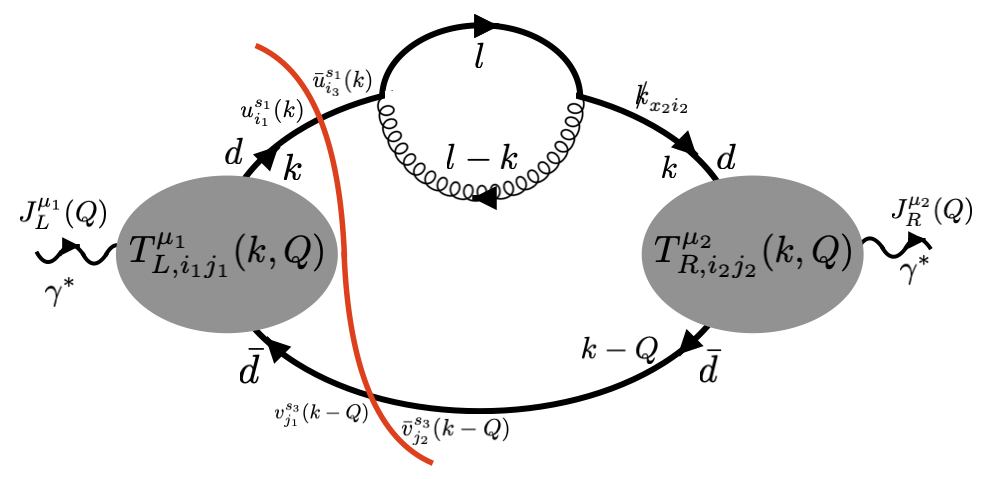
\includegraphics[width=1\linewidth]{CA.png}}
\end{minipage}\hfill
\begin{minipage}{0.5\linewidth}
\centering
{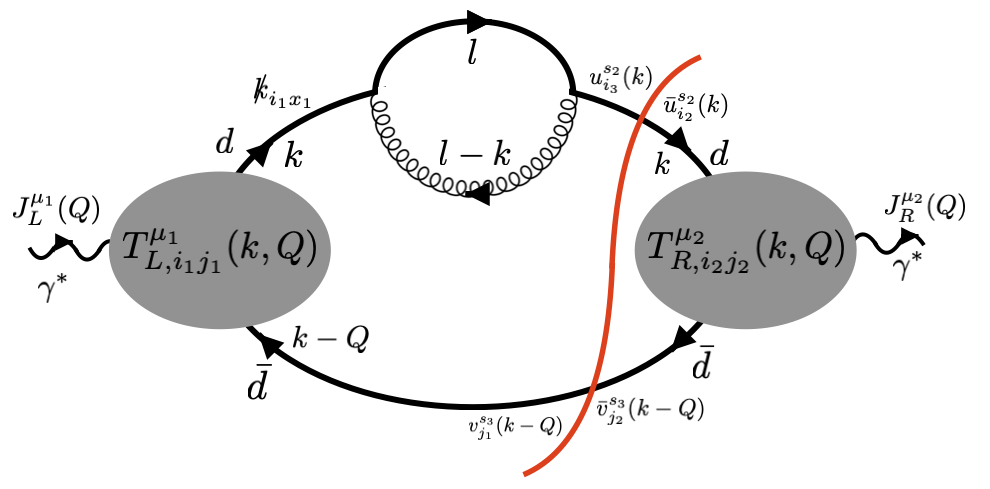
\includegraphics[width=1\linewidth]{CB.png}}
\end{minipage}
{\caption{\label{CAB} Cutkosky contributions C$_\textrm{A}$ (left) and C$_\textrm{B}$ (right).}}
\end{center}
\end{figure}
\noindent where each Cutkoski cut of a four-momentum $q$ translates into the expression $(-2\pi i)\delta^{+}\left(q^2\right)$.
We can now write explicitly the contributions C$_\textrm{A}$ and C$_\textrm{B}$ as:
\begin{eqnarray}
\label{CABdef}
{\textrm{C}}_{\textrm{A}}&=& (-2\pi i)^2 \delta^{+}\left((k-Q)^2\right)\delta^{+}\left(k^2\right)  \sum_{s_1 \in \pm} \sum_{s_3 \in \pm} 
\left( T^{L}_{i_1 j_1} v^{s_3}_{j_1} u^{s_1}_{i_1} \right )
\left( \bar{u}^{s_1}_{i_3} \Sigma^{R}_{i_3 x_2}(k,l) \frac{(-i)\slashed{k}_{x_2 i_2}}{k^2+i\delta} T^{R}_{i_2 j_2} \bar{v}^{s_3}_{j_2} \right) \nonumber\\
{\textrm{C}}_{\textrm{B}}&=& (-2\pi i)^2 \delta^{+}\left((k-Q)^2\right)\delta^{+}\left(k^2\right) \sum_{s_2 \in \pm} \sum_{s_3 \in \pm} 
\left( T^{L}_{i_1 j_1}  \frac{(i)\slashed{k}_{i_1 x_1}}{k^2-i\delta} \Sigma^{L}_{x_1 i_3}(k,l) u^{s_2}_{i_3} v^{s_3}_{j_1} \right )
\left( \bar{u}^{s_2}_{i_2}  T^{R}_{i_2 j_2} \bar{v}^{s_3}_{j_2} \right) \nonumber\\
\end{eqnarray}
with $T_{ij}\equiv J^\mu(k,Q) T^\mu_{ij}(k,Q)$ and where we kept implicit the dependences of the polarization vectors in the loop momenta.
The self-energy factors $\Sigma^{L/R}$ are defined as:
\begin{eqnarray}
\Gamma^{R}_{ij} (k) &\equiv& (-i) (\slashed{k}_{i j} ) + \left( \int \frac{\tilde{d}l}{(2\pi)^4} \Sigma^{R}_{ix} (k,l) \right)  (-i) (\slashed{k}_{x j} ) \nonumber\\
\Gamma^{L}_{ij} (k) &\equiv& (i) (\slashed{k}_{i j} ) + (i) (\slashed{k}_{i x} ) \left(\int \frac{\tilde{d}l}{(2\pi)^4} \Sigma^{L}_{x j}(k,l) \right)
\end{eqnarray}
where  $\int \tilde{d}l\; \equiv \left(\frac{\mu^2}{4\pi e^{-\gamma}}\right)^{\epsilon} \int \frac{d^{4-2\epsilon}l}{(2\pi)^{-2\epsilon}} $. When setting all couplings to 1, the explicit expressions of $\Sigma^{R/L}_{ij}$ then reads:
\begin{eqnarray}
\label{Fdefinitions}
B^R_{i_1 i_2}(k,l)&=& \left( \sum_{s_1 \in \pm} u^{s_1}_{i_1}(k) \bar{u}^{s_1}_{i_3}(k) \right) \Sigma^{R}_{i_3 x_2}(k,l)\frac{ (-i)\slashed{k}_{x_2 i_2}}{k^2-i\delta} \nonumber\\ 
&=& 2 C_F (1-\epsilon) [(i)(-i)(i)(i)](-i) \frac{ (-\slashed{k}\slashed{l}\slashed{k})_{i_3 i_2} }{(k^2-i\delta)(l^2-i\delta) ((l-k)^2-i\delta)} \nonumber\\
&=& 2 C_F (1-\epsilon) (-i) \frac{ (\slashed{k}\slashed{l}\slashed{k})_{i_1 i_2} }{(k^2-i\delta) (l^2-i\delta) ((l-k)^2-i\delta)} 
= 2 C_F (1-\epsilon) \mathcal{F}^R_{i_1i_2}(k,l))
\nonumber\\
B^L_{i_1 i_2}(k,l)&=& \frac{(i)\slashed{k}_{i_1 x_1}}{k^2+i\delta} \Sigma^{L}_{x_1 i_3}(k,l) \left( \sum_{s_2 \in \pm} u^{s_2}_{i_3}(k)\bar{u}^{s_2}_{i_2}(k)  \right) \nonumber\\
&=& 2 C_F (1-\epsilon) (i)[(-i)(i)(-i)(-i)] \frac{ (-\slashed{k}\slashed{l}\slashed{k})_{i_1 i_2} }{ (k^2+i\delta) (l^2+i\delta) ((l-k)^2+i\delta)}\nonumber\\
&=& 2 C_F (1-\epsilon) (i) \frac{ (\slashed{k}\slashed{l}\slashed{k})_{i_1 i_2} }{(k^2+i\delta) (l^2+i\delta) ((l-k)^2+i\delta)} 
= 2 C_F (1-\epsilon)  \mathcal{F}^L_{i_1i_2}(k,l)),
\nonumber \\  
\end{eqnarray}
where the $C_F$ terms comes from having performed the colour algebra.
Our target expression from eq.~\ref{CABdef} cannot be evaluated explicitly given that it is proportional to $\delta^{+}\left(k^2\right)/k^2$.
To address this issue, we will take advaxntage of the dispersion relation which we introduce in the next section.

\section{Dispersive representation}

Any function $f(x)$ and analytic in $\mathbb{C}\setminus(-\infty,-x^\star)\cup(x^\star,\infty)$ can be written using Cauchy's theorem by performing an integral along the contours indicated in fig.~\ref{IntegrationContours} below with $q^0\equiv x$ and $|\vec{q}|\equiv x^\star$:
\begin{figure}[ht!]
\begin{center}
\begin{minipage}{0.65\linewidth}
\centering
{\caption{\label{IntegrationContours} Integration contours considered for deriving the dispersion relation.}}
{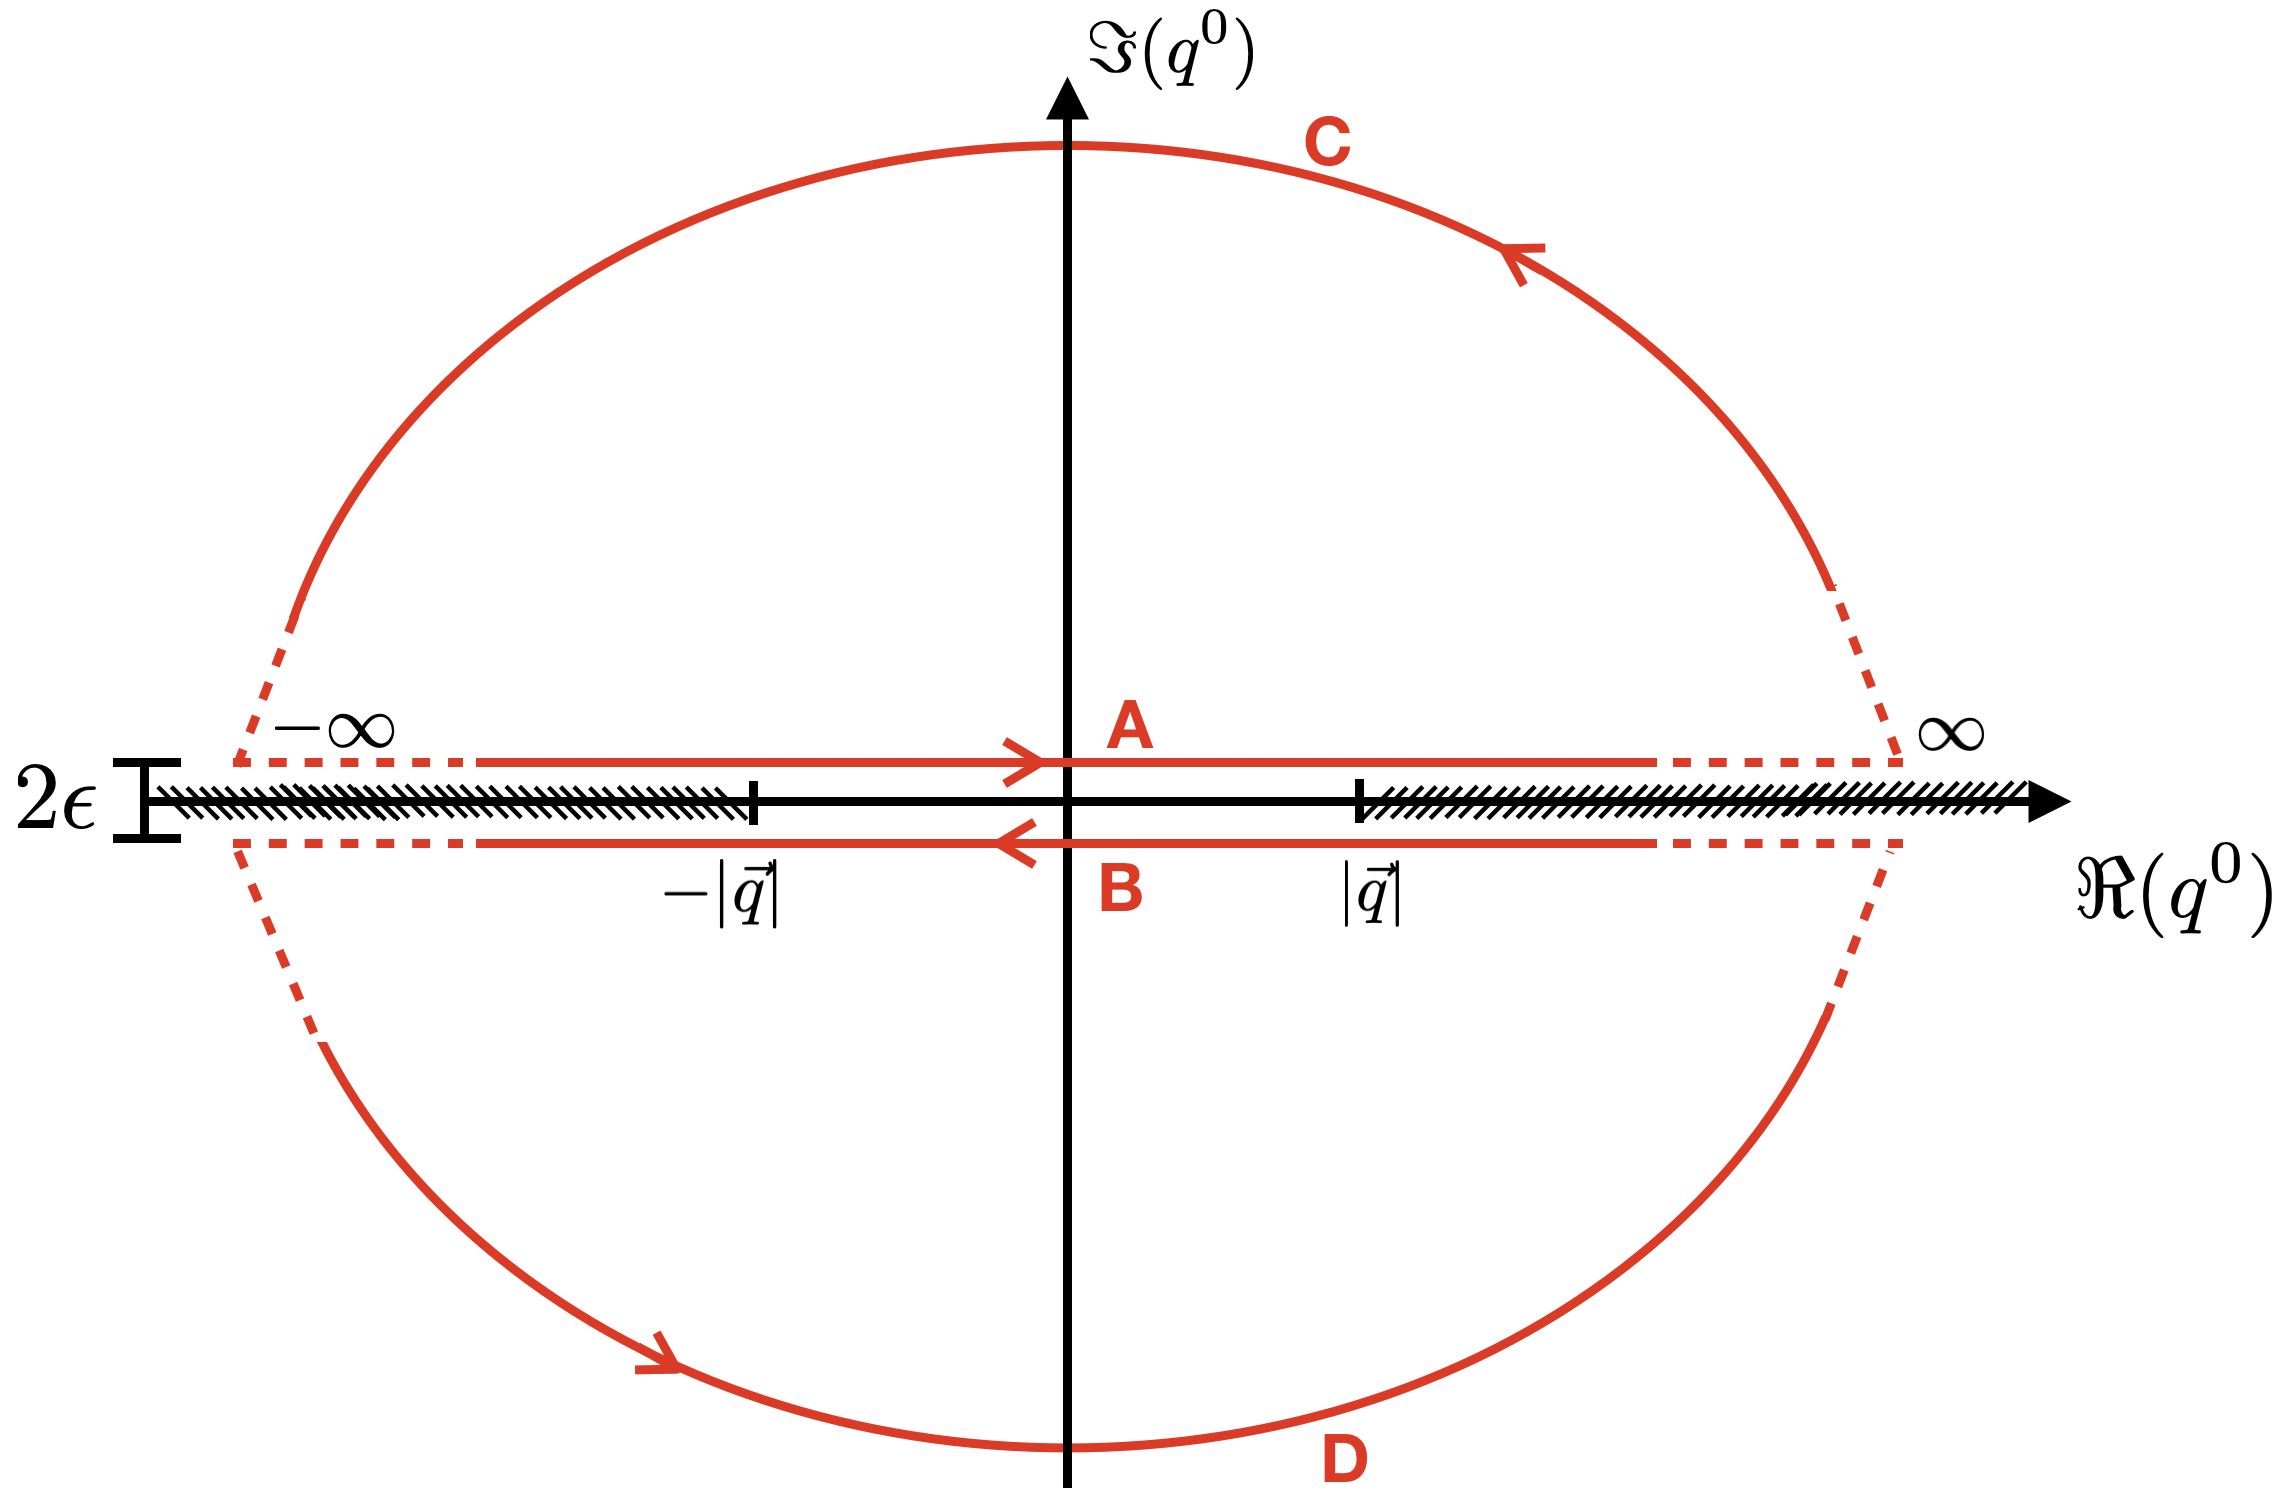
\includegraphics[width=0.75\linewidth]{integration_contour.png}}
\end{minipage}\hfill
\end{center}
\end{figure}
yielding the following dispersive expression for $f(x)$:
\begin{eqnarray}
f(x)&=& \lim_{\epsilon \rightarrow 0^+}\frac{1}{2\pi i} \left[ 
\underbrace{ \int_{-\infty}^\infty d z \frac{ f(z+i\epsilon) }{z-x+i\epsilon} }_{\textrm{segment A}} +
\underbrace{ \int_{\infty}^{-\infty} d z \frac{ f(z-i\epsilon) }{z-x-i\epsilon} }_{\textrm{segment B}}
\right ] \nonumber \\
&=& 
\frac{1}{2\pi i}  \lim_{\epsilon \rightarrow 0^+} \int_{-\infty}^\infty d z \frac{f(z+i\epsilon) - f(z-i\epsilon)   }{z-x} \nonumber \\
&=&
\frac{1}{2\pi i} \int_{-\infty}^\infty d z \frac{ \textrm{disc} \left[ f(z) \right] }{z-x}
=\frac{1}{2\pi i} \int_{0}^\infty d z \left[ \frac{ \textrm{disc} \left[ f(z) \right] }{z-x}-\frac{ \textrm{disc} \left[ f(-z) \right] }{z+x}\right]
,\label{DispertionRelation}
\end{eqnarray}
where we neglected the $\pm i \epsilon$ in the denominators of the second line because we assume that $f(s)$ is analytic everywhere except on $(-\infty,-x^\star)\cup(x^\star,\infty)$ which our contour never crosses. 
We also used the assumption\footnote{Notice that for this assumption to hold, it will be important that we include the denominator $\frac{1}{k^2}$ in the definition of $\mathcal{F}^{L/R}$ in eq.~\ref{Fdefinitions}. We stress that this property is then completely independent of whether or not one has performed UV renormalisation at this stage.} that $\lim_{|z| \rightarrow \infty} f(z) = 0$, allowing us to neglect the segments C and D of the contour at infinity. Finally, we find it useful to split the integration domain in the last line of eq.~\ref{DispertionRelation} so as to be able to integrate over only positive $z$ values.

We now consider applying eq.~\ref{DispertionRelation} to the particular case of both functions $\mathcal{F}^L_{i_1i_2}(k^0,\vec{k},l)$ and $\mathcal{F}^R_{i_1i_2}(k^0,\vec{k},l)$, and considering $x\equiv k^0$.
We will also take advantage of the fact that self-energy functions satisfy (at any order in perturbation theory and also for massive internal lines (?) ) the reality condition known as the \emph{Schwartz reflection principle}, namely:
\begin{equation}
\mathcal{F}^{L/R}_{i_1i_2}(z^*, \vec{k},l)=\mathcal{F}^{L/R}_{i_1i_2}(z, \vec{k},l)^*
\end{equation}
which allows us to rewrite the discontinuity as:
\begin{eqnarray}
\textrm{disc} \left[ \mathcal{F}^{L/R}_{i_1i_2}(z, \vec{k},l) \right] &=& \lim_{\epsilon->0^+} \left( \mathcal{F}^{L/R}_{i_1i_2}(z+i\epsilon, \vec{k},l) - \mathcal{F}^{L/R}_{i_1i_2}(z-i\epsilon, \vec{k},l) \right ) \nonumber \\
&=&  \lim_{\epsilon \rightarrow 0^+} \left( \mathcal{F}^{L/R}_{i_1i_2}(z+i\epsilon, \vec{k},l) - \mathcal{F}^{L/R}_{i_1i_2}(z+i\epsilon, \vec{k},l)^* \right )\nonumber \\
&=&  2 i \lim_{\epsilon \rightarrow 0^+}  \Im{ \left[ \mathcal{F}^{L/R}_{i_1i_2}(z+i\epsilon, \vec{k},l) \right] } \nonumber \\
&=&  i \sum_{\textrm{C}^+_i\in \mathcal{C}_\mathcal{F}^{L/R}} \textrm{C}^+_i\left[ \mathcal{F}^{L/R}_{i_1i_2}(z, \vec{k},l)\right ],
\label{DiscIntoCutkosky}
\end{eqnarray}
where $\mathcal{C}_\mathcal{F}^{L/R}$ denote the list of Cutkosky cuts the integral $\mathcal{F}^{L/R}$ is subject to while the application of the \emph{signed} Cutkosky operator $C^{\pm}_i$ appearing on the last line reads:
\begin{equation}
C^{\pm}_i = (\mp2\pi i)^{|\textrm{cuts}_i|} \prod_{j\in \textrm{cuts}_i} q_j^2(z) \delta^{\pm}\left(q_j^2(z)\right)
\end{equation}
({\bf WARNING:} at this stage it seems that the above Cutkosky rule should \emph{not} involve a complex conjugation on the expression of the graph sitting on the right-hand side of the cut!).
We note that the last equality in eq.~\ref{DiscIntoCutkosky} stems from the Cutkosky rule that expresses the discontinuity of loop integrals, as written in Eq. (55) of ref.~\cite{Zwicky:2016lka}.
Also, for a complete unknown reason {\bf{HELP HERE!}}, the discontinuity of $\mathcal{F}^{L}$ is only non-zero for \emph{positive} energy $k^0$ while $\mathcal{F}^{R}$ only contributes to the discontinuity at a \emph{negative} $k^0$.
We thus arrive at the following final expression for the re-expression of $\mathcal{F}^{L/R}$ as quantities we will denote $\mathcal{\tilde{F}}^{R}$ and that are computed through the dispersive relation:
\begin{eqnarray}
\label{dispertionRelationApplied}
\mathcal{\tilde{F}}^{L}_{i_1i_2}(k^0, \vec{k},l) = \frac{1}{2\pi} \int_{0}^\infty d z \frac{ \sum_{\textrm{C}^+_i\in\mathcal{C}_\mathcal{F}^{L}} \textrm{C}^+_i\left[ \mathcal{F}^{L}_{i_1i_2}(z, \vec{k},l)\right ] }{z-k^0} \nonumber\\
\mathcal{\tilde{F}}^{R}_{i_1i_2}(k^0, \vec{k},l) = -\frac{1}{2\pi} \int_{0}^\infty d z \frac{ \sum_{\textrm{C}^-_i\in\mathcal{C}_\mathcal{F}^{R}} \textrm{C}^-_i\left[ \mathcal{F}^{R}_{i_1i_2}(-z, \vec{k},l)\right ] }{z+k^0} \nonumber\\
\end{eqnarray} 
\emph{PS:} Ideally one should be able to ditch the "dispersive" representation and find a way to arrive at the same expressions starting from the two-loop vacuum diagram formed by the one-loop bubble with the external leg closed onto itself:
\begin{figure}[ht!]
\begin{center}
\begin{minipage}{0.75\linewidth}
\centering
{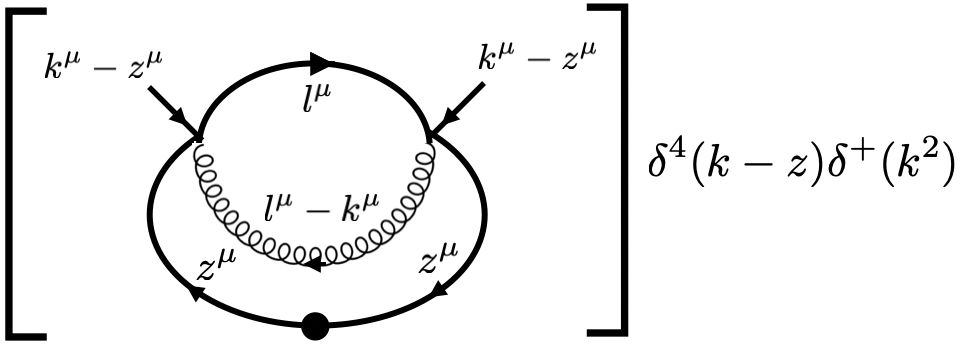
\includegraphics[width=1\linewidth]{LTD_instead_of_dispersive.png}}
\end{minipage}\hfill
{\caption{\label{DispersiveAlternative} Possible alternative representation of the dispersive representation that could be entirely derived within our LTD framework.}}
\end{center}
\end{figure}
Then maybe one could proceed like for normal two-loop LTD and finally impose $\delta^4(z-k)\delta(k^2)$ on the final expression, although it is not clear how to do so at this stage...
\section{Direct evaluation}

We now turn to directly evaluating the two expressions of Eq.~\ref{dispertionRelationApplied}. 
A first thing to note is that the set of cuts in $\mathcal{C}_\mathcal{F}^{L/R}$ are identical, except for their sign, in both the $L$ and $R$ contributions and it reads:
\begin{equation}
\mathcal{C}_\mathcal{F}^{L/R} \equiv \{ (2\pi i)^2 (l^2) (l-k)^2 \delta^{+/-}\left(l^2\right)\delta^{+/-}\left((l-k)^2\right)\}
\end{equation}
It is also worth noting that it is important that we do not consider further complex conjugation in the application of the Cutkosky operator above, as this would yield an extra incorrect minus sign in contribution $\textrm{C}_\textrm{B}$ of fig.~\ref{CAB}. The lack of complex conjugation in the application of these \emph{bubble Cutkosky cuts} also implies that the sign of the causal prescription involved in the contributions $\mathcal{F}^{L/R}_{i_1 i_2}$ remains unchanged!

It is useful at this stage to provide a graphical representation of the dispersion relation of eq.~\ref{dispertionRelationApplied} combined with the overall contributions ${\textrm{C}}_{\textrm{A}}$ and ${\textrm{C}}_{\textrm{B}}$ of fig.~\ref{CAB}:
\begin{figure}[ht!]
\begin{center}
\begin{minipage}{0.5\linewidth}
\centering
{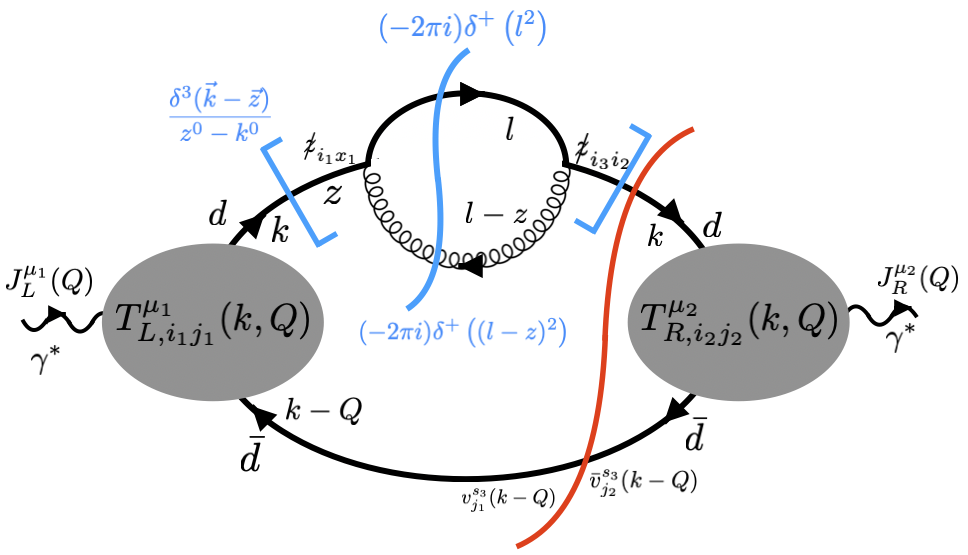
\includegraphics[width=1\linewidth]{CA_bubble_cut.png}}
\end{minipage}\hfill
\begin{minipage}{0.5\linewidth}
\centering
{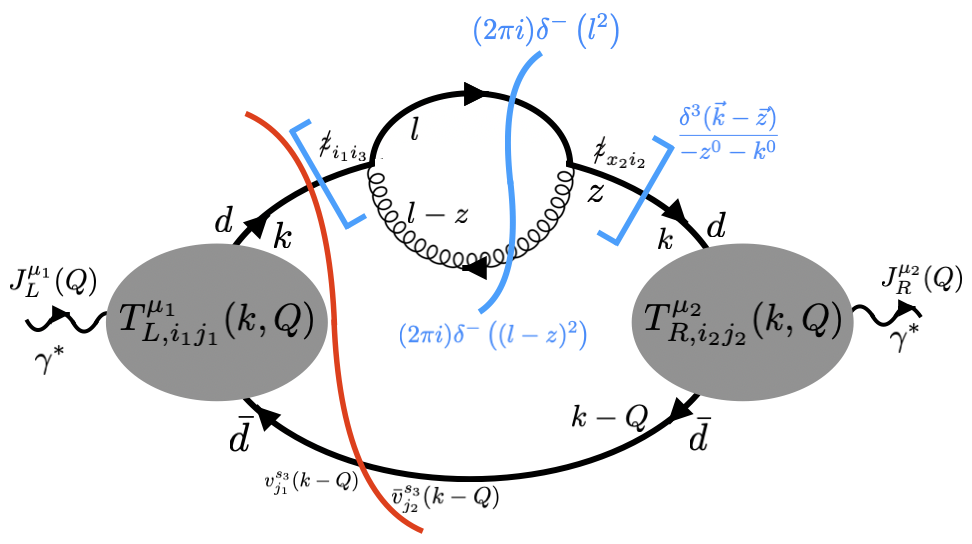
\includegraphics[width=1\linewidth]{CB_bubble_cut.png}}
\end{minipage}
{\caption{\label{CABwithBubbleCuts} Contributions C$_\textrm{A}$ (left) and C$_\textrm{B}$ (right), including bubble cuts (in blue) stemming from the dispersive representation of eq.~\ref{dispertionRelationApplied}. The squared blue cut indicate a break in the energy conservation between $z^\mu=(z,\vec{k})$ and $k^\mu=(k^0,\vec{k})$.}}
\end{center}
\end{figure}
Pay attention in particular how the polarization vectors $u_{i_1}^{s_1}(k)$ and $\bar{u}_{i_2}^{s_2}(k)$ have been pulled \emph{inside} the expression of the bubble subject to the dispersive representation. This implies that the momentum dependency in these polarisation vectors changes from $k$ to $z$, thus allowing us to simplify the polarisation sum into $\slashed{z}_{i_3 i_2}$ and $\slashed{z}_{i_1 i_3}$ respectively, as done in eq.~\ref{Fdefinitions}.

We are now ready to explicitly compute $\mathcal{\tilde{F}}^{L}_{i_1i_2}(k^0, \vec{k},l)$ as in eq.~\ref{dispertionRelationApplied}, while also pulling in the integration measure $\int \frac{\tilde{d} l}{(2\pi)^4}$ and swapping the order of integration with $\int d z$:
\begin{eqnarray}
\label{CBexplicit}
\textrm{C}_\textrm{B}\left(k \right) &=& \underbrace{T^{L}_{j_1 i_1} (\slashed{k}-\slashed{Q})_{j_2 j_1} T^{R}_{i_2 j_2} 2 C_F (1-\epsilon)  }_{T_{i_2 i_1}(k,Q,\epsilon)}  \int \frac{\tilde{d} l}{(2\pi)^4} \mathcal{\tilde{F}}^{L}_{i_1i_2}(k^0, \vec{k},l) \nonumber\\
&=&T_{i_2 i_1}  \int \frac{\tilde{d} l}{(2\pi)^4}  \frac{1}{2\pi} \int_{0}^\infty d z^0 \frac{ \sum_{\textrm{C}^+_i\in\mathcal{C}_\mathcal{F}^{L}} \textrm{C}^+_i\left[ \mathcal{F}^{L}_{i_1i_2}(z^0, \vec{k},l)\right ] }{z^0-k^0} \nonumber \\
&=&T_{i_2 i_1}  \int \frac{\tilde{d}^3 \vec{l}}{(2\pi)^4}  \frac{(-2\pi i)^2}{2\pi} \int_{0}^\infty d z^0 \frac{1}{z^0-k^0} \frac{(i)\slashed{z}\slashed{l}\slashed{z}}{z^2 (2 |\vec{l}|) (2 |\vec{l}-\vec{k}|)} \delta \left(z^0-|\vec{l}|-|\vec{l}-\vec{k}|\right), \nonumber \\
\end{eqnarray}
with $z\equiv(z^0,\vec{k})$.
For $\textrm{C}_\textrm{A}$ we get:
\begin{eqnarray}
\label{CAexplicit}
\textrm{C}_\textrm{A}\left(k \right) &=& T_{i_2 i_1} \int \frac{\tilde{d} l}{(2\pi)^4} \mathcal{\tilde{F}}^{R}_{i_1i_2}(k^0, \vec{k},l)\nonumber\\
&=&T_{i_2 i_1}  \int \frac{\tilde{d} l}{(2\pi)^4}  \frac{1}{2\pi} \int_{0}^\infty d z^0 \frac{ \sum_{\textrm{C}^-_i\in\mathcal{C}_\mathcal{F}^{R}} \textrm{C}^-_i\left[ \mathcal{F}^{R}_{i_1i_2}(-z^0, \vec{k},l)\right ] }{z^0-k^0} \nonumber \\
&=&T_{i_2 i_1}  \int \frac{\tilde{d}^3 \vec{l}}{(2\pi)^4}  \frac{(2\pi i)^2}{2\pi} \int_{0}^\infty d z^0 \frac{1}{-z^0-k^0} \frac{(-i)\slashed{\bar{z}}\slashed{\bar{l}}\slashed{\bar{z}}}{\bar{z}^2 (-2 |\vec{l}|) (-2 |\vec{l}-\vec{k}|)} \delta \left(-z^0+|\vec{l}|+|\vec{l}-\vec{k}|\right) \nonumber \\
\end{eqnarray}
with $\bar{z}\equiv(-z^0,\vec{k})$ and $\bar{l}\equiv(-l^0,\vec{l})$.
When combining $\textrm{C}_\textrm{A}$ and $\textrm{C}_\textrm{B}$ we find:
\begin{eqnarray}
\textrm{C}_\textrm{B}+ \textrm{C}_\textrm{A} &=& (-i)T_{i_2 i_1}  \int \frac{\tilde{d}^3 \vec{l}}{(2\pi)^3} \int_{0}^\infty d z^0 \frac{\delta \left(z^0-|\vec{l}|-|\vec{l}-\vec{k}|\right)}{(z^0)^2-(k^0)^2} \frac{1}{(2 |\vec{l}|) (2 |\vec{l}-\vec{k}|)} \nonumber \\
&\times&\left( 
\frac{z^0+k^0}{z^2} \slashed{z}\slashed{l}\slashed{z} + \frac{z^0-k^0}{\bar{z}^2} \slashed{\bar{z}}\slashed{\bar{l}}\slashed{\bar{z}}
\right)
\end{eqnarray}
Since $z^2=\bar{z}^2$ 
% and also that:
%\begin{eqnarray}
%\slashed{\bar{z}}\slashed{\bar{l}}\slashed{\bar{z}}&=&(-z^0\gamma^0+\vec{k} \cdot \vec{\gamma}) \slashed{l} (-z^0\gamma^0+\vec{k} \cdot \vec{\gamma}) \nonumber\\
%&=&\slashed{z}\slashed{l}\slashed{z}- 2 z^0\left( \gamma^0 \slashed{l} (\vec{k} \cdot \vec{\gamma}) + (\vec{k} \cdot \vec{\gamma}) \slashed{l} \gamma^0 \right) \nonumber\\
%&=&-\slashed{z}\slashed{l}\slashed{z} + 2 (z^0)^2 \gamma^0 \slashed{l} \gamma^0 + 2 (\vec{k} \cdot \vec{\gamma}) \slashed{l} (\vec{k} \cdot \vec{\gamma}),
%\end{eqnarray}
we write the final expression for $\textrm{C}_\textrm{B}+ \textrm{C}_\textrm{A}$ by performing the integration over $z^0$ with $\delta \left(z^0-|\vec{l}|-|\vec{l}-\vec{k}|\right)$ and introducing the variable $z^\star \equiv |\vec{l}|+|\vec{l}-\vec{k}|$:
%\begin{eqnarray}
%\label{OurFinalOffshellExpressionSelfEnergy}
%&& \textrm{C}_\textrm{B}+ \textrm{C}_\textrm{A} = (-i)T_{i_2 i_1}  \nonumber\\
%&& \times \int \frac{\tilde{d}^3 \vec{l}}{(2\pi)^3}
%\frac{
%z^\star \left( 2 (z^\star)^2 \gamma^0 \slashed{l} \gamma^0 + 2 (\vec{k} \cdot \vec{\gamma}) \slashed{l} (\vec{k} \cdot \vec{\gamma}) \right) +
%k^0 \left (
%2 z^\star\left( \gamma^0 \slashed{l} (\vec{k} \cdot \vec{\gamma}) + (\vec{k} \cdot \vec{\gamma}) \slashed{l} \gamma^0 \right)
%\right) 
%}{
%\left( (z^\star)^2-(k^0)^2 \right) \left( (z^\star)^2-|\vec{k}|^2\right) \left( 2 |\vec{l}|\; 2 |\vec{l}-\vec{k}| \right) } \nonumber\\
%\end{eqnarray}
\begin{eqnarray}
\label{OurFinalOffshellExpressionSelfEnergy}
&& \textrm{C}_\textrm{B}+ \textrm{C}_\textrm{A} = (-i)T_{i_2 i_1} \int \frac{\tilde{d}^3 \vec{l}}{(2\pi)^3}
\frac{
(z^\star+k^0) \slashed{z}\slashed{l}\slashed{z} + (z^\star-k^0)  \slashed{\bar{z}}\slashed{\bar{l}}\slashed{\bar{z}}
}{
\left( (z^\star)^2-(k^0)^2 \right) \left( (z^\star)^2-|\vec{k}|^2\right) \left( 2 |\vec{l}|\; 2 |\vec{l}-\vec{k}| \right) } \nonumber\\
\end{eqnarray}
When considering the case of an external bubble (as in fig.~\ref{CABwithBubbleCuts}), we can pull in the Cutkosky cut $(-2\pi i)\delta^2\left(k^2\right)$ which simplifies the above a bit as follows:
%\begin{eqnarray}
%\label{OurFinalExpressionSelfEnergy}
%&& \left( \textrm{C}_\textrm{B}+ \textrm{C}_\textrm{A}\right) (-2\pi i)\delta^2\left(k^2\right) = \frac{(-2\pi i)}{2|\vec{k}|}(-i)T_{i_2 i_1}  \nonumber\\
%&& \times \int \frac{\tilde{d}^3 \vec{l}}{(2\pi)^3}
%\frac{
%z^\star \left( 2 (z^\star)^2 \gamma^0 \slashed{l} \gamma^0 + 2 (\vec{k} \cdot \vec{\gamma}) \slashed{l} (\vec{k} \cdot \vec{\gamma}) \right) +
%|\vec{k}| \left (
%2 z^\star\left( \gamma^0 \slashed{l} (\vec{k} \cdot \vec{\gamma}) + (\vec{k} \cdot \vec{\gamma}) \slashed{l} \gamma^0 \right)
%\right) 
%}{
%\left( (z^\star)^2-|\vec{k}|^2\right)^2 \left( 2 |\vec{l}|\; 2 |\vec{l}-\vec{k}| \right) }. \nonumber\\
%\end{eqnarray}
\begin{eqnarray}
\label{OurFinalExpressionSelfEnergy}
&& \left( \textrm{C}_\textrm{B}+ \textrm{C}_\textrm{A}\right) (-2\pi i)\delta^2\left(k^2\right) = \frac{(-2\pi i)}{2|\vec{k}|}(-i)T_{i_2 i_1}  \int \frac{\tilde{d}^3 \vec{l}}{(2\pi)^3}
\frac{
(z^\star+|\vec{k}|) \slashed{z}\slashed{l}\slashed{z} + (z^\star-|\vec{k}|)  \slashed{\bar{z}}\slashed{\bar{l}}\slashed{\bar{z}}
}{
\left( (z^\star)^2-|\vec{k}|^2\right)^2 \left( 2 |\vec{l}|\; 2 |\vec{l}-\vec{k}| \right) } \nonumber\\
\end{eqnarray}
As we can see, the above expression of the quark self-energy is not as elegant as eq.(336) of Soper's Beowulf notes, because we did not choose a smart momentum routing allowing him to perform the Lorentz algebra shown in his eq.(331).
This implies that we could not explicitly cancel the $\left( (z^\star)^2-|\vec{k}|^2\right)$ denominator in eq.~\ref{OurFinalOffshellExpressionSelfEnergy} (which is not formally necessary, for example Soper also does not cancel it in the case of the self-energy of the gluon). 
However, our expression of eq.~\ref{OurFinalExpressionSelfEnergy} is formally equivalent to Soper's one, as explicitly shown in the Mathematica notebook accompanying these notes.

The expression of eq.~\ref{OurFinalExpressionSelfEnergy} has a superficial degree of UV divergence in $|\vec{l}|$ of $7-6=1$ (as in Soper's case) which therefore calls for local UV counterterms cancelling both the leading \emph{and subleading} UV behaviour and reproducing the on-shell renormalisation conditions of eqs.~\ref{renormConditionsA}-\ref{renormConditionsD}.
This is the object of the next section. 

\section{UV local counterterms}

In this section, we aim at designing local UV counterterms for the contributions $\mathcal{\tilde{F}}^{L}_{i_1i_2}(k^0, \vec{k},l)$ and $\mathcal{\tilde{F}}^{R}_{i_1i_2}(k^0, \vec{k},l)$.
We will denote these counterterms $\mathcal{\bar{F}}^{L}_{i_1i_2}(k^0, \vec{k},l)$ and $\mathcal{\bar{F}}^{R}_{i_1i_2}(k^0, \vec{k},l)$ respectively and they must be designed so as satisfy the following properties (remember that $\slashed{k}\slashed{k}=k^2$):
\begin{itemize}
\item C1) $\lim_{|\vec{l}|\rightarrow \infty} |\vec{l}|^3 \left[ \mathcal{\tilde{F}}^{L/R}_{i_1i_2}(k^0, \vec{k},l) - \mathcal{\bar{F}}^{L/R}_{i_1i_2}(k^0, \vec{k},l) \right] =0$
\item C2) $\lim_{k^0\rightarrow |\vec{k}|} \slashed{k} \int \tilde{d}l \left[ \mathcal{\tilde{F}}^{L}_{i_1i_2}(k^0, \vec{k},l) - \mathcal{\bar{F}}^{L}_{i_1i_2}(k^0, \vec{k},l) \right] =0$ (from eq.~\ref{renormConditionsA})
\item C3) $\lim_{k^0\rightarrow |\vec{k}|} \int \tilde{d}\;l \left[ \mathcal{\tilde{F}}^{R}_{i_1i_2}(k^0, \vec{k},l) - \mathcal{\bar{F}}^{R}_{i_1i_2}(k^0, \vec{k},l) \right] \slashed{k} =0$ (from eq.~\ref{renormConditionsB})
\item C4) $\lim_{k^0\rightarrow |\vec{k}|} \int \tilde{d} \left[ \mathcal{\tilde{F}}^{L}_{i_1i_2}(k^0, \vec{k},l) - \mathcal{\bar{F}}^{L}_{i_1i_2}(k^0, \vec{k},l) \right] =0$ (directly from eq.~\ref{renormConditionsC})
\item C5) $\lim_{k^0\rightarrow |\vec{k}|} \int \tilde{d} \left[ \mathcal{\tilde{F}}^{R}_{i_1i_2}(k^0, \vec{k},l) - \mathcal{\bar{F}}^{R}_{i_1i_2}(k^0, \vec{k},l) \right] =0$ (directly from eq.~\ref{renormConditionsD})
\end{itemize}
We already see here an apparent difference w.r.t Soper's approach where he insists on enforcing the following on his UV counterterm:
\begin{equation}
\lim_{k^0\rightarrow |\vec{k}|} \int \tilde{d}l \mathcal{\bar{F}}^{L/R}_{i_1i_2}(k^0, \vec{k},l) = 0,
\end{equation}
which would correspond to the $\overline{\textrm{MS}}$ renormalisation conditions (as he claims himself) which I believe are not appropriate in the context of the renormalisation of external self-energies. But it may be that this makes not difference in the case of massless quarks since we know that their wavefunction UV counterterms have no finite piece \emph{also} in the on-shell scheme. This would however definitely make a difference for massive quarks (a.k.a top-quark).

In order to separate the task of satisfying condition C1) and that of satisfying eqs. C2)$\rightarrow$C5), we will write our counterterms as:
\begin{equation}
\mathcal{\bar{F}}^{L/R}_{i_1i_2} = \mathcal{\hat{F}}^{L/R}_{i_1i_2}+\Delta \mathcal{\bar{F}}^{L/R}_{i_1i_2},
\end{equation}
where
\begin{eqnarray}
&&\lim_{|\vec{l}|\rightarrow \infty} |\vec{l}|^3 \Delta \mathcal{\bar{F}}^{L/R}_{i_1i_2}(k^0, \vec{k},l) = 0 \\
&&\lim_{k^0\rightarrow |\vec{k}|} \int \tilde{d} \Delta \mathcal{\bar{F}}^{L/R}_{i_1i_2}(k^0, \vec{k},l) = 
\lim_{k^0\rightarrow |\vec{k}|} \int \tilde{d} \left[ \mathcal{\tilde{F}}^{L/R}_{i_1i_2}(k^0, \vec{k},l) - \mathcal{\hat{F}}^{L/R}_{i_1i_2}(k^0, \vec{k},l) \right]. \label{constraintOnDeltaF}
\end{eqnarray}
In other terms, the role of $\mathcal{\hat{F}}^{L/R}_{i_1i_2}$ is to guarantee on its own that C1) is satisfied while the role of $\Delta \mathcal{\bar{F}}^{L/R}_{i_1i_2}$ is \emph{only} to insure that eqs. C2)$\rightarrow$C5) are satisfied.\\

In this section, we will focus only on designing $\mathcal{\hat{F}}^{L/R}_{i_1i_2}$.
We first note that it would be simple to design such counterterm if we could start from a clear four-dimensional picture similar to that of Fig.~\ref{DispersiveAlternative}.
Unfortunately, our current understanding of the relation between LTD and the dispersive formula does not allow us to do this and we must start from the last line of eq.~\ref{CBexplicit}, where the integration over $l^0$ has already be performed.
Within the dispersive approach we can only consider the UV behaviour *after* this energy integration as otherwise the UV divergence due to the apparition of $z^0$ in the denominator would not be manifest.
Our starting expression to approximate is therefore:
\begin{equation}
\textrm{C}_\textrm{B}\left(k \right) =
T_{i_2 i_1}  \int \frac{\tilde{d}^3 \vec{l}}{(2\pi)^3} (-i) \frac{1}{z^\star-k^0} \frac{\slashed{z}\slashed{l}\slashed{z}}{z^2 (2 |\vec{l}|) (2 |\vec{l}-\vec{k}|)},
\end{equation}
with $z^\star = |\vec{l}|+|\vec{l}-\vec{k}|$ and $z=(z^\star,\vec{k})$. Since the integrand goes like $|\vec{l}|^{-2}$ we will need to subtract \emph{both} the leading and subleading UV limit for condition C1) to be satisfied.
The brute force way to proceed is to write $\vec{l}=t\;\vec{\hat{l}}$ thus obtaining:
\begin{eqnarray}
 |\vec{l}|&=&t\sqrt{\hat{\vec{l}} \cdot  \hat{\vec{l}}} \\
 |\vec{l}-\vec{k}|&=&\sqrt{t^2\; \hat{\vec{l}} \cdot  \hat{\vec{l}}-t\; 2\hat{\vec{l}} \cdot \vec{k} + \vec{k} \cdot \vec{k}}.
 \end{eqnarray}
We can then expand the resulting expression in $t$ and retain all terms up to (and including) $\mathcal{O}(t^{-3})$.
Even though this would certainly be a valid candidate for $\mathcal{\hat{F}}^{L/R}_{i_1i_2}$, it is not clear how it relates to the one obtained by Soper and also whether we could easily accommodate the resulting denominators as "normal propagators" fitting our Rust implementation of the bubble problem.

\section{Matching renormalisation conditions}
In this section, we carry out the computing of the quantities $\Delta \mathcal{\bar{F}}^{L/R}_{i_1i_2}$.\\

{\bf{TODO: In principle this should "simply" amount to integrating eq.~\ref{constraintOnDeltaF} in dimensional regularisation and reverse-engineering a local expression integrating to that quantity... I don't see a systematic way of doing this however. Maybe contact Soper on the matter...
We should of course not forget however that we can always decide to add the integrated contribution of $\Delta \mathcal{\bar{F}}^{L/R}_{i_1i_2}$ through an additional form-factor of the lower-order super graph.
}}

\section{LSZ}
\label{sec:LSZ}

The $LTD^2$ formalism should be matched with the common way of calculating scattering amplitudes between asymptotic states. The most used framework is currently the LSZ formalism, which establishes that the contribution of self-energy corrections of external particles on the scattering amplitude only amount to a constant. For a scattering of an even number of fermions, the LSZ formula reads
\begin{equation}
\langle S \rangle(p_1,...,p_n; \ p_{n+1},...,p_{n+m})=\lim_{p_1^0\rightarrow E_1}...\lim_{p_{m+n}^0\rightarrow E_{m+n}} Z_\psi^{\frac{n+m}{2}}\Bigg(\prod_{i=1}^{n+m}\frac{1}{Z_\psi}\frac{\slashed{p}_i -m_\text{p}}{\slashed{p}_i -m_0-\Sigma(p)}\Bigg)\Gamma_{\text{amp}},
\end{equation}
where $\Gamma_{\text{amp}}$ is the amputated $m+n$ point function, $m_0$ and $m_\text{p}$ are the bare and physical mass respectively, $Z_\psi$ the field renormalization factor.
If the onshell scheme is carried out for the renormalization of the external self-energy corrections, then the formula simplifies considerably and one obtains
\begin{equation}\label{lsz2}
\langle S \rangle(p_1,...,p_n; \ p_{n+1},...,p_{n+m})=Z_\psi^{\frac{n+m}{2}}\Gamma_{\text{amp}}\big|_{p_i^2=m^2}.
\end{equation}
Unfortunately, it is impossible for us to carry out the program as laid out by this simple equation: indeed, the self-energy corrections have IR divergences which need to locally cancel with their real counter-parts in order for the integrand to be fully locally finite. Extracting the IR divergent part while, at the same time, ensuring matching with the LSZ formula, is of vital importance in order to obtain the correct result. 

Recall that after renormalization, the fermion propagator has the form   
\begin{equation}
\frac{1}{Z_\psi}\frac{1}{\slashed p -m_0-\Sigma(p)}=\frac{1}{\slashed p -m_\text{r}-\Sigma_R(p)},
\end{equation}
with
\begin{equation}
\label{eq:definingRenormSigma}
\Sigma_R(p)=\Sigma(p)+m_\text{r} \delta Z_m - (\slashed p - m_\text{r})\delta Z_\psi,
\end{equation}
and $m_0=Z_m m_\text{r}$, $Z_m=1+\delta Z_m$ and $Z_\psi=1+\delta Z_\psi$. An easy way to reproduce \eqref{lsz2} is to impose the onshell scheme, in which $m_\text{r}=m_\text{p}$ and $\Sigma_R(p)=0$. As already mentioned, we cannot impose these conditions right away, since $\Sigma_R(p)$ still contains an IR divergence, which should locally be cancelled with a real emission singularity. However, we can start by imposing the renormalized mass to be the same as the physical mass; this is equivalent to requiring that
\begin{equation}\label{onshell1}
\Sigma_R(p^2=m_\text{p}^2)=0.
\end{equation}
This condition fixes the value of $\delta Z_m$. Having done this, the Dyson sum can be unfolded again
\begin{equation}
\frac{1}{\slashed p -m_\text{r}-\Sigma_R(p)}=\frac{1}{\slashed p -m_\text{p}}\Bigg(1+\sum_n \Bigg(\frac{\Sigma_R(p)}{\slashed p -m_\text{p}}\Bigg)^n\Bigg).
\end{equation}

It is now necessary to extract the IR-divergent part of the 1PI. First, out of self-consistency, one should expect the IR divergent part to not be contained in $\Sigma_R(p^2=m_\text{p}^2)$, since it was already set to vanish. Indeed, this is the case. Using the definition of finite part, which extracts any finite element of an integral carried out in dimensional regularization a part from the $\epsilon_{\text{uv}}$ or $\epsilon_{\text{ir}}$ poles, it is possible to define a finite 1PI
\begin{equation}
\tilde\Sigma_R(p)=\text{finite}(\Sigma_R(p)),
\end{equation} 
which allows to write
\begin{align}
\frac{1}{\slashed p -m_\text{r}-\Sigma_R(p)}=\frac{1}{\slashed p -m_\text{p}}\Bigg(1+\sum_n \Bigg(\frac{\tilde\Sigma_R(p)}{\slashed p -m_\text{p}}\Bigg)^n\Bigg)+S_{\text{ir}}, \\
S_{\text{ir}}=\frac{1}{\slashed p -m_\text{p}}\sum_n \Bigg[\Bigg(\frac{\Sigma_R(p)}{\slashed p -m_\text{p}}\Bigg)^n-\Bigg(\frac{\tilde\Sigma_R(p)}{\slashed p -m_\text{p}}\Bigg)^n\Bigg].
\end{align}
$S_{\text{ir}}$ contains the infrared pole part which is to be cancelled with the real counterpart. Thus, it can be simply ignored with respect to the matching with the LSZ formula. In particular, it will cancel even before the onshell limit is taken (one can imagine to express it in terms of a parameter gauging how close we are to being on shell, and a parameter being the dimensional regulator). The comparison of what remains with \eqref{lsz2} then yields
\begin{equation}
\lim_{p^0\rightarrow E_p}\frac{\tilde\Sigma_R(p)}{\slashed p -m_\text{p}}=0.
\end{equation} 
Expanding up to first order in the vanishing onshell parameter
\begin{equation}
\frac{\tilde\Sigma_R(p)}{\slashed p -m_\text{p}}=\frac{\tilde\Sigma_R(p^2=m_\text{p}^2)}{\slashed p -m_\text{p}}+\frac{\slashed p +m_\text{p}}{p^0+E_p}\frac{d\tilde\Sigma_R}{dp^0}+o(p^0-E_p).
\end{equation} 
and thus we re-obtain the onshell renormalization conditions
\begin{align}\label{onshell2}
\tilde\Sigma_R(p^2=m_\text{p}^2)=0 \\ \label{onshell3}
\frac{d\tilde\Sigma_R}{dp^0}=0.
\end{align}
The first observation is that the procedure of extracting IR divergences is consistent, since $\tilde\Sigma_R(p^2=m_\text{p}^2)=\Sigma_R(p^2=m_\text{p}^2)$ and thus \eqref{onshell1} is equivalent to \eqref{onshell2}. In order to reproduce \eqref{onshell3}, instead, one can write
\begin{equation}
\frac{d\Sigma_R}{dp^0}=\Bigg(\frac{d\Sigma_R}{dp^0}-\frac{d\tilde\Sigma_R}{dp^0}\Bigg)+\frac{d\tilde\Sigma_R}{dp^0}
\end{equation}
which is ultimately the object of interest, and that which we will express locally in order to preserve local IR cancellations, and then satisfy the onshell condition by writing
\begin{equation}\label{cond}
\frac{d\Sigma_R}{dp^0}=\Bigg[\frac{d\Sigma}{dp^0}-\text{CT}_\text{uv}\Bigg[\frac{d\Sigma}{dp^0}\Bigg]\Bigg]_{d=4}-\Bigg[\text{finite}\Bigg(\frac{d\Sigma}{dp^0}\Bigg)-\text{finite}\Bigg(\text{CT}_\text{uv}\Bigg[\frac{d\Sigma}{dp^0}\Bigg]\Bigg)\Bigg]_d.
\end{equation}
Indeed, the renormalization condition is satisfied, since
\begin{equation}
\frac{d\tilde\Sigma_R}{dp^0}=\text{finite}\Bigg(\frac{d\Sigma_R}{dp^0}\Bigg)=0.\end{equation}
In practice, how is this formula embedded in the $LTD^2$ formalism? The first part of \eqref{cond},
\begin{equation}
\Bigg[\frac{d\Sigma_R}{dp^0}\Bigg]_{\substack{\text{numerically}\\ \text{computed}}}=\Bigg[\frac{d\Sigma}{dp^0}-\text{CT}_\text{uv}\Bigg[\frac{d\Sigma}{dp^0}\Bigg]\Bigg]_{d=4}
\end{equation}
 can be evaluated numerically, since it will be UV finite and it's IR divergence will locally cancel with the real counterpart. Then, one will need to add back the finite part, which will make the overall contribution of the bubble exactly equal to what's strictly needed to cancel the IR divergences, that is
  \begin{equation}
\Bigg[\frac{d\Sigma_R}{dp^0}\Bigg]_{\substack{\text{analitically}\\ \text{computed}}}=-\Bigg[\text{finite}\Bigg(\frac{d\Sigma}{dp^0}\Bigg)-\text{finite}\Bigg(\text{CT}_\text{uv}\Bigg[\frac{d\Sigma}{dp^0}\Bigg]\Bigg)\Bigg]_d.
\end{equation}

The fixed renormalization constants are
\begin{align}
m_\text{p} \delta Z_m=\Sigma(p^2=m_\text{p}^2) \\
\delta Z_\psi =\frac{\slashed p + m_\text{p}}{p^0+E_p}\Bigg[\frac{d\Sigma}{dp^0}-\frac{d\Sigma_R}{dp^0}\Bigg]
\end{align}


\section{Formal expression of the matching terms $\Delta \textrm{UV}_{m,\psi}$}
\label{sec:formalDeltaUV}

We can now start from~\eqref{eq:definingRenormSigma} and insert zero as follows as well as a correction factor $\Delta \textrm{UV}_m + (p^0-\sqrt{|\vec{p}|+m^2})\Delta \textrm{UV}_2$ which will need to be adjusted in order to reproduce the desired renormalisation conditions which induced the renormalisation counterterms $\delta Z_m$ and $\delta Z_\psi$:
\begin{eqnarray}
\Sigma_R(p)&=&\Sigma(p)-m_\text{r} \delta Z_m - (\slashed p - m_\text{r})\delta Z_\psi +  {\Bigg [ } \label{eq:UVCTdefa}\\
&&
-\underbrace{\left( \int d^{4-2\epsilon}k\; \textrm{UVCT}(k,p){\Big |}_{d=4} \right)}_{\textrm{Will be combined with $\Sigma(p)$}} 
+ \underbrace{\left( \int d^{4-2\epsilon}k\; \textrm{UVCT}(k,p){\Big |}_{d=4-2\epsilon} \right)}_{\textrm{Complete d-dimensional integral of UVCT}}
 \label{eq:UVCTdefb}\\
&&- 
\underbrace{\left [ 
\int d^{4-2\epsilon}k\; \textrm{UVCT}(k,p){\Big |}_{d=4-2\epsilon} -  \left( \int d^{4-2\epsilon}k\; \textrm{UVCT}(k,p){\Big |}_{d=4} \right) \label{eq:UVCTdefc} 
\right ]}_{\textrm{R-terms}} \\
&{\Bigg ] }&
\end{eqnarray}
Then, writing $\Sigma_{\textrm{UV-subtracted}}\equiv \Sigma(p)-\left( \int d^{4-2\epsilon}k\; \textrm{UVCT}(k){\Big |}_{d=4} \right)$ and collectively denoting rational terms as R-terms, we have:
\begin{eqnarray}
\Sigma_R(p)&=&\Sigma_{\textrm{UV-subtracted}}(p)+m_\text{r} \delta Z_m - (\slashed p - m_\text{r})\delta Z_\psi -\textrm{R-terms} \nonumber\\
&&
+ \int d^{4-2\epsilon}k\; \textrm{UVCT}(k,p){\Big |}_{d=4-2\epsilon} 
 \label{eq:SigmaRenormalaLTD}
\end{eqnarray}
The quantity we are including in our numerical computation reads as follows:
\begin{equation}
\Sigma^{(\textrm{LTD})}(p) = \left( 
\underbrace{\Sigma^{(\textrm{LTD})}_{m} (p)}_{
\equiv 0
}
+ \Delta \textrm{UV}_m \right) 
+ (p^0-\sqrt{|\vec{p}|+m^2}) {\Big(}
\underbrace{
\Sigma^{(\textrm{LTD})}_{\psi} (p)
}_{
\frac{\partial}{\partial p^0} \Sigma_{\textrm{UV-subtracted}}(p)
}
+ \Delta \textrm{UV}_\psi {\Big)}.
\end{equation}
We now want to determine the expressions of $\Delta \textrm{UV}_m$ and $\Delta \textrm{UV}_\psi$ that reproduce the OS renormalisation conditions given our particular choices for $\Sigma^{(\textrm{LTD})}_{m} (p)$ and $\Sigma^{(\textrm{LTD})}_{\psi} (p)$.
We do so by imposing $\Sigma_R(p)=\Sigma^{(\textrm{LTD})}(p)$ on both on-shell conditions listed in Eqs.~\eqref{onshell2}. For the $\Delta \textrm{UV}_m$ correction factor, we recall that we choose $ \Sigma^{(\textrm{LTD})}_{m} (p) \equiv 0$, so that in particular $\Sigma^{(\textrm{LTD})}_{m} (p^2=m_p^2)=0 $, and we immediately find:
\begin{eqnarray}
&&\Sigma_R(p^2=m_p^2) = 0 = \Sigma^{(\textrm{LTD})}(m_p^2)  = \underbrace{\Sigma^{(\textrm{LTD})}_{m} (m_p^2)}_{=0} + \Delta \textrm{UV}_m \nonumber \\
&\rightarrow& \Delta \textrm{UV}_m = 0.
\end{eqnarray}
Now $\Delta\textrm{UV}_\psi$ is then obtained by looking at the OS renormalisation condition on the derivative of the renormalised self-energy:
\begin{eqnarray}
\frac{\partial}{\partial p^0} \Sigma_R \Big|_{p^2=m_p^2} = 0 &=& 
\frac{\partial}{\partial p^0} \Sigma_{\textrm{UV-subtracted}}(p) {\Big|}_{p^2=m_p^2}
- \gamma^0 \delta Z_\psi  \nonumber\\
&&
+ \frac{\partial}{\partial p^0}\int d^{4-2\epsilon}k\; \textrm{UVCT}(k,p){\Big |}_{d=4-2\epsilon, p^2=m_p^2 }  -\frac{\partial}{\partial p^0}\textrm{R-terms}|_{p^2=m_p^2}  \nonumber \\
\frac{\partial}{\partial p^0} \Sigma^{(\textrm{LTD})}(p) {\Big|}_{p^2=m_p^2} &=& 
\Sigma^{(\textrm{LTD})}_{\psi} (p) {\Big|}_{p^2=m_p^2} + \Delta \textrm{UV}_\psi  \nonumber \\
&=& \frac{\partial}{\partial p^0} \Sigma_{\textrm{UV-subtracted}}(p){\Big|}_{p^2=m_p^2} + \Delta \textrm{UV}_\psi,
\end{eqnarray}
and imposing $\frac{\partial}{\partial p^0} \Sigma^{(\textrm{LTD})}(p) {\Big|}_{p^2=m_p^2} = \frac{\partial}{\partial p^0} \Sigma_R \Big|_{p^2=m_p^2}  = 0$ then yields the expression for $\Delta UV_\psi$:
\begin{eqnarray}
&& \frac{\partial}{\partial p^0} \Sigma_{\textrm{UV-subtracted}}(p){\Big|}_{p^2=m_p^2} + \Delta \textrm{UV}_\psi =
\frac{\partial}{\partial p^0} \Sigma_{\textrm{UV-subtracted}}(p) {\Big|}_{p^2=m_p^2}
- \gamma^0 \delta Z_\psi  \nonumber\\
&&
+ \frac{\partial}{\partial p^0}\int d^{4-2\epsilon}k\; \textrm{UVCT}(k,p){\Big |}_{d=4-2\epsilon, p^2=m_p^2 }  -\frac{\partial}{\partial p^0}\textrm{R-terms}|_{p^2=m_p^2}  \nonumber \\
&\rightarrow& \Delta \textrm{UV}_\psi = -\frac{\partial}{\partial p^0}\textrm{R-terms}|_{p^2=m_p^2}  + \left[
\frac{\partial}{\partial p^0} \int d^{4-2\epsilon}k\; \textrm{UVCT}(k,p){\Big |}_{d=4-2\epsilon, p^2=m_p^2 }
- \gamma^0 \delta Z_\psi
\right ] \nonumber \\
\label{eq:DeltaUVpsidef}
\end{eqnarray}
Notice that the expression in squared brackets is finite only if one considers poles of \emph{UV origin only} in $\delta Z_\psi$. This is typically not the case as the "UV-finite" part of $\delta Z_\psi$ contains IR poles which would then appear in $ \Delta \textrm{UV}_\psi $.
We are however free to ignore these poles.
To understand why, one can perform the thought experiment of thinking about local IR counterterms to regularise the remaining IR divergences in $\Sigma_{\textrm{UV-subtracted}}(p)$.
These would allow us to really integrate the self-energy separately from the real-emission contributions which we left out of the present discussion.
However, these local IR counterterms would also need to be analytically integrated in dimensional regularisation and added back as an additional term $\left [ \textrm{CT}_{\textrm{IR}} \right ]_{d=4-2\epsilon}$ in the expression of $ \Delta \textrm{UV}_\psi $ in~\eqref{eq:DeltaUVpsidef}.
There are many possible choices for the functional form of the local counterterm $\textrm{CT}_{\textrm{IR}}$ (i.e. it must only reproduce the original integrand in the IR limits, but can have arbitrary additional non-diverging contributions in that limit), but the only forms that \emph{directly} match our formalism of local cancellation of IR divergences between real-emission and virtual contributions realised in LTD$^2$ are the ones for which the integrated counterpart $\left [ \textrm{CT}_{\textrm{IR}} \right ]_{d=4-2\epsilon}$ has only IR poles and \emph{no finite part}, thus justifying how its inclusion simply amounts to ignoring the pole of IR origin in $\delta Z_\psi$.

\section{Explicit one-loop expression of the one-loop matching terms $\Delta \textrm{UV}_{\psi}$ for a massless fermion}
\label{sec::explicitDeltaUV}

In this section, we give an explicit expression for the quantity $\Delta \textrm{UV}_{\psi}$ of eq.~\eqref{eq:DeltaUVpsidef} for the case of the one-loop self-energy correction of a massless fermion (sitting on the left of the Cutkosky cut):
We start by writing explicitly $\Sigma(p)$ as:
\begin{equation}
\Sigma_{ij}(p) \delta_{i_1 i_2} = (-i g_s) (i) (-i g_s )(-i ) C_F \delta_{i_1 i_2} \gamma_{i x_1}^\mu {\Big(} 
\underbrace{
\int \frac{d k}{(2\pi)^4} \frac{\slashed{k}_{x_1 x_2}}{k^2 (k-p)^2}
}_{\overline{\Sigma}_{x_1 x_2}(p)}
\Big{)} g^{\mu\nu}\gamma^\nu_{x_2 j}
\end{equation}
for which the first derivative in $p^0$ reads:
\begin{eqnarray}
\frac{\partial}{\partial p^0} \overline{\Sigma}_{ij}(p)
&=&\int \frac{d k}{(2\pi)^4} \frac{\partial}{\partial p^0} \frac{\slashed{k}_{x_1 x_2}}{k^2 (k-p)^2} \nonumber \\
&=& \int \frac{d k}{(2\pi)^4} \frac{ \slashed{k}_{x_1 x_2}(k^0-p^0) }{k^2 \left[(k-p)^2\right]^2}.
\end{eqnarray}
We will now build the local UV counterterm by taking the limit $p^0=0$ and $\vec{p}=\vec{0}$ and providing the denominator with a UV mass $M_\textrm{UV}$ in order to screen all IR divergences. We hence obtain:
\begin{equation}
\textrm{UVCT}(k,p) \equiv \textrm{UVCT}(k) = \frac{ \slashed{k}_{x_1 x_2} k\cdot\eta }{\left[ k^2-M_\textrm{UV}^2\right]^3},
\end{equation}
where $\eta^\mu=(1,0,0,0)$. We are therefore interested in computing in dimensional regulation the following integral:
\begin{eqnarray}
&&\int \frac{\tilde{d} k}{(2\pi)^4} \textrm{UVCT}(k) = \gamma^\mu \eta^\nu A^{\mu\nu} \nonumber\\ 
&&A^{\mu\nu} = \int \frac{\tilde{d} k}{(2\pi)^4} \frac{ k^\mu k^\nu }{\left[ k^2-M_\textrm{UV}^2\right]^3}, \label{Adef}
\end{eqnarray}
where  $\int \tilde{d}k\; \equiv \left(\frac{\mu^2}{4\pi e^{-\gamma}}\right)^{\epsilon} \int \frac{d^{4-2\epsilon}k}{(2\pi)^{-2\epsilon}} $ (the additional factor $ \left(\frac{1}{4\pi e^{-\gamma}}\right)^{\epsilon} $ is designed so as to automatically reabsorb into a redefinition of the renormalisation scale the terms removed by finite part of the $\overline{\textrm{MS}}$ renormalisation counterterms). 
We can now contract $A^{\mu\nu}$ with its only tensor decomposition allowed by Lorentz invariance, that is: $A^{\mu\nu}=A g^{\mu\nu}$ and $A=\frac{1}{d}g^{\mu\nu}A^{\mu\nu}$.
The form factor $A$ can then easily be computed as follows:
\begin{eqnarray}
A&=&\frac{1}{d} \int \frac{\tilde{d} k}{(2\pi)^4} \frac{ k^2 }{\left[ k^2-M_\textrm{UV}^2\right]^3} \nonumber\\
&=&\frac{1}{d} \left [ 
\int\frac{\tilde{d} k}{(2\pi)^4} \frac{ 1 }{\left[ k^2-M_\textrm{UV}^2\right]^2} 
-M_\textrm{UV}^2 \int \frac{\tilde{d} k}{(2\pi)^4} \frac{ 1 }{\left[ k^2-M_\textrm{UV}^2\right]^3} 
\right ].
\end{eqnarray}
With the help of the following result (see for instance eq.~(3) of ref.~\cite{Steinhauser:2000ry}):
\begin{equation}
\int \frac{d^d k}{(2\pi)^d} \frac{ 1 }{\left[ k^2+M^2\right]^a} =\frac{(M^2)^{\frac{d}{2}-a}}{(4\pi)^\frac{d}{2}}\frac{\Gamma(a-\frac{d}{2})}{\Gamma(a)}
\end{equation}
we find:
\begin{eqnarray}
A&=&\frac{1}{4-2\epsilon}\left(\frac{\mu^2}{4\pi e^{-\gamma}}\right)^{\epsilon} \frac{(-M_\textrm{UV}^2)^{\frac{4-2\epsilon}{2}-2}}{(4\pi)^\frac{d}{2}} \left [ 
\frac{\Gamma(2-\frac{4-2\epsilon}{2})}{\Gamma(2)} - \frac{\Gamma(3-\frac{4-2\epsilon}{2})}{\Gamma(3)}
\right] \nonumber \\
&=&\frac{1}{4-2\epsilon} \frac{1}{(4\pi)^2}\left(\frac{\mu^2}{-M_\textrm{UV}^2 e^{-\gamma}}\right)^{\epsilon}\left [ 
\frac{\Gamma(\epsilon)}{\Gamma(2)} - \frac{\Gamma(1+\epsilon)}{\Gamma(3)}
\right] 
\end{eqnarray}
which we can expand to order $\mathcal{O}(\epsilon)$ to find:
\begin{equation}
A=\frac{1}{64\pi^2}\left[ \frac{1}{\epsilon} + \log{\frac{\mu^2}{-M_\textrm{UV}^2}} \right].
\end{equation}
This leaves us with the computation of the rational terms which we can obtain by separating the $\epsilon-dimensional$ pieces of both the numerator (yielding $R_1$ and the denominator which yields $R_2$).
In order to do so we will introduce a new notation based on the decomposition of all Lorentz vectors onto an orthonormal basis with four basis vectors $\hat{e}_i$ and an $(d-4)$-dimensional set of directions $\hat{\tilde{e}}_i$:
\begin{equation}
\bar{k} = k_i \hat{e}_i + \tilde{k}_i \hat{\tilde{e}}_i,
\end{equation}
where the bar notation serves to denote d-dimensional vectors and tilde $(d-4)$-dimensional ones. 
The orthonormality of the basis imposes $\hat{e}_i \cdot \hat{\tilde{e}}_j = 0\; \forall i,j$.
Using this decomposition, we can now also define an equivalent $(d-4)$-dimensional part of numerators and denominators:
\begin{eqnarray}
&&\bar{N}(\bar{k})=N(k)+\tilde{N}(\tilde{k}^2,k,\epsilon) \nonumber\\
&&\bar{D}_i = \bar{q}_i^2+m^2 = q_i^2+\tilde{q}_i^2+m^2 = D_i + \tilde{q}_i^2.
\end{eqnarray}
In our particular case we have $\bar{N}(\bar{k})=\bar{k}^2$ and therefore $N(k)=k^2$ and $\tilde{N}(\tilde{k}^2,k,\epsilon)=\tilde{k}^2$.
We will also make use of the following identity:
\begin{equation}
\frac{1}{\bar{D}_i}=\frac{Z_i}{D_i},\textrm{  } Z_i=1-\frac{\tilde{q}_i^2}{\bar{D}_i}
\end{equation}
We can first attempt at computing the rational piece directly with the following integral:
\begin{eqnarray}
A_{R} &=& \int \frac{\tilde{d} k}{(2\pi)^4} \left [
\frac{1}{d} \frac{ \bar{k}^2 }{\left[ \bar{k}^2-M_\textrm{UV}^2\right]^3}
-\frac{1}{4} \frac{ \bar{k}^2-\tilde{k}^2  }{\left[ \bar{k}^2-\tilde{k}^2-M_\textrm{UV}^2\right]^3}
\right] \nonumber\\
&=& \int \frac{\tilde{d} k}{(2\pi)^4}
{\Big[} 
\frac{\left(\frac{1}{d}-\frac{1}{4}\right)\bar{k}^2}
{\left[ \bar{k}^2-M_\textrm{UV}^2\right]^3}
+\frac{\frac{1}{4}\tilde{k}^2\left(2\bar{k}^2 +M_\textrm{UV}^2 \right)
}{\left[ \bar{k}^2-M_\textrm{UV}^2\right]^4} 
+\frac{\frac{1}{4}3(\tilde{k}^2)^2\left(\bar{k}^2 +M_\textrm{UV}^2 \right)
}{\left[ \bar{k}^2-M_\textrm{UV}^2\right]^5} \nonumber\\
&&+\mathcal{O}\left(\frac{(\tilde{k}^2)^3(A\bar{k}^2+B)}{\left[ \bar{k}^2-M_\textrm{UV}^2\right]^6}\right)
{\Big]}
\end{eqnarray}
But there is no cutoff as all these terms give a contribution so.... I must be doing something wrong...
Next attempt is then to expand around $k^2$ and not $\bar{k}^2$ in the numerator.

Recalling the definition of $\Delta \textrm{UV}_\psi$ from~\eqref{eq:DeltaUVpsidef}:
\begin{equation}
\Delta \textrm{UV}_\psi = -\frac{\partial}{\partial p^0}\textrm{R-terms}|_{p^2=m_p^2}  + \left[
\frac{\partial}{\partial p^0} \int d^{4-2\epsilon}k\; \textrm{UVCT}(k,p){\Big |}_{d=4-2\epsilon, p^2=m_p^2 }
- \gamma^0 \delta Z_\psi
\right ],
\end{equation}
we can insert the expression of $\delta Z_\psi$ without its IR pole, together with our newly found expressions for the other quantities and obtain \emph{WARNING: below must be adjusted once we have a final version of the $A_R$ expression!}:
\begin{eqnarray}
\Delta \textrm{UV}_{\psi,ij} \delta_{i_1 i_2} &=& -g_s^2 C_F \delta_{i_1 i_2} \left[ 
\gamma_{i x_1}^\mu
\gamma_{x_1 x_2}^0 \frac{1}{64\pi^2}\left(
-(-\frac{1}{2}-1)+
\frac{1}{\epsilon} + \log{\frac{\mu^2}{-M_\textrm{UV}^2}}
\right)
g^{\mu\nu}\gamma_{x_2 j}^\nu
\right] \nonumber \\
&&- \gamma^0_{ij} \left( \frac{g_s^2}{32\pi^2} C_F \frac{1}{\epsilon_{\textrm{UV}}} \right),
\end{eqnarray}
and if we now choose $M_\textrm{UV}^2=\mu^2$ and use the identity $\gamma^\mu \gamma^\nu \gamma^\mu=(2-d) \gamma^\nu$, we get:
\begin{equation}
\Delta \textrm{UV}_{\psi,ij} \delta_{i_1 i_2} = g_s^2 C_F \delta_{i_1 i_2} \gamma^0_{ij} \left( 
\frac{3}{64\pi^2}
\right),
\end{equation}
and with $\alpha_s=\frac{g_s^2}{4\pi}$ and $C_F=\frac{4}{3}$, we eventually get:
\begin{equation}
\Delta \textrm{UV}_{\psi,ij} \delta_{i_1 i_2} = \left( \delta_{i_1 i_2} \gamma^0_{ij} \frac{\alpha_s}{\pi} \right) \left(\frac{1}{4}\right), 
\end{equation}
we can recognise the inclusive NLO cross-section in the first parenthesis and therefore write:
\begin{equation}
\sigma_{\Delta \textrm{UV}_{\psi}} = \left(+\frac{1}{4}\right) \sigma_{\textrm{NLO}}.
\end{equation}
Finally we recall that for our current numerical implementation to be correct, we require $\sigma_{\Delta \textrm{UV}_{\psi}}\sim +96$ [pb]. Since we have $\sigma_{\textrm{NLO}}=290.8$ [pb], the above formula gives us $72.7$ [pb].
The correct result must instead be a prefactor of $\frac{1}{3}$ which would nicely yield $97$ [pb].
\section{Computation of Tadpoles}
In the following we denote $\tilde{k}$ as $k_{[\epsilon]}$, $\bar{k}$ as $k_{[D]}$ and $k$ as $k_{[4]}$, to make the dimensional dependence clear. We start by considering the integral 
\begin{align}
	I_1=\int \frac{\text{d}^D k_{[D]}}{(2 \pi)^4} \frac{k_{[\epsilon]}^2}{D^n} ,
\end{align}
where $D=k_{[4]}^2+k_{[\epsilon]}^2+M_{UV}^2$.
Rewriting this integral yields
\begin{align}
	I_1 &=\int \frac{\text{d}^D k_{[D]}}{(2 \pi)^4} \frac{k_{[\epsilon]}}{D^n} \\
		&=\int \frac{\text{d}^4 k_{[4]}}{(2 \pi)^4} \text{d }^{-2\epsilon} k_{[\epsilon]} \frac{k_{[\epsilon]}^2}{D^n} \\
		&=\int \frac{\text{d}^4 k_{[4]}}{(2 \pi)^4} \underbrace{\int \text{d}\Omega_{-2\epsilon-1}}_{=:V_{-2\epsilon-1}} \int_{0}^{\infty}  \frac{\text{d} r_{\epsilon}}{2} r^{\frac{-2\epsilon-2}{2}}\frac{r_{\epsilon}}{D^n}
\end{align}
with $r_{\epsilon}=k_{[\epsilon]}^2$ and we are allowed to go to spherical coordinates, since the propagator is quadratic in $k_{\epsilon}$. However, recognizing that
\begin{align}
\int \text{d}^{2-2 \epsilon} k_{[\epsilon]}	= V_{-2\epsilon+1}\int_{0}^{\infty}\frac{\text{d} r_{\epsilon}}{2} r^{-\epsilon} , 
\end{align}
we see that
\begin{align}
	I_1 &=\int \frac{\text{d}^D k_{[D]}}{(2 \pi)^4} \frac{k_{[\epsilon]}}{D^n} \\
		&= \frac{V_{-2\epsilon-1}}{V_{-2\epsilon+1}}\int \frac{\text{d}^4 k_{[4]}}{(2 \pi)^4} \int \text{d}^{2-2 \epsilon} k_{[\epsilon]} \frac{1}{D^n} \\
		&=\frac{V_{-2\epsilon-1}}{V_{-2\epsilon+1}}\underbrace{\int \frac{\text{d}^{D+2} k_{[D+2]}}{(2 \pi)^4} \frac{1}{D^n}}_{=:I_n(D+2)}. \label{eq:I1}
\end{align}
In particular, that means we can relate it to a higher dimensional tadpole by include the volumina of n-ball
\begin{align}
	V_D=\frac{2\pi^{\frac{D+1}{2}}}{\Gamma\left(\frac{D+1}{2}\right)}.
\end{align}
The generalization of \eqref{eq:I1} to arbitrary even insertions of $k_{[\epsilon]}^{2l}$ is straight-forward:
\begin{align}
	I_l=\frac{V_{-2\epsilon-1}}{V_{-2\epsilon+2l}} I_n(D+2l)
\end{align}
by iteration and by expressing $k_{[4]}^2=D-k_{[\epsilon]}^2-M_{UV}^2$ every possible integral of that type will evaluate to linear combinations of tadpoles weighted by volumina of the corresponding $n$-balls. Computations of this type and many more algebraic properties of the explicit dimensional splitting are explained in \cite{Gnendiger:2017pys}.
\bibliographystyle{JHEP}
\bibliography{biblio}


\section{Legacy}

We are now ready to compute the two rational pieces:
\begin{eqnarray}
A_{R_2}&=& \frac{1}{d} \int \frac{\tilde{d} k}{(2\pi)^4} \frac{ \tilde{k}^2 }{\left[ \bar{k}^2-M_\textrm{UV}^2\right]^3} \nonumber \\
A_{R_1} &=& \frac{1}{d} \int \frac{\tilde{d} k}{(2\pi)^4} \frac{ \bar{k}^2 Z^3 - k^2 }{\left[ k^2-M_\textrm{UV}^2\right]^3}
= \frac{1}{d} \int \frac{\tilde{d} k}{(2\pi)^4} \frac{ \bar{k}^2 \left( -3\frac{\tilde{k}^2}{\bar{D}_i} +\mathcal{O}\left((\tilde{k}^2)^2\right) \right) }{\left[ k^2-M_\textrm{UV}^2\right]^3} \nonumber \\
&=&  -\frac{3}{d} \int \frac{\tilde{d} k}{(2\pi)^4} \frac{ \bar{k}^2 \tilde{k}^2 }{\left[ \bar{k}^2-M_\textrm{UV}^2\right]^4} +\mathcal{O}\left((\tilde{k}^2)^2\right).
\end{eqnarray}
Then, using the result of the first line of eq.(A.2) and of the third line of eq.(A.3) of ref.~\cite{Draggiotis:2009yb} (adjusted to our normalisation and to the Euclidean case):
\begin{eqnarray}
\int d^d \bar{k} \frac{\tilde{k}^2}{\left( \bar{k}^2-M^2 \right)^3}=-\frac{\textrm{i}\pi^2}{2}\frac{1}{(2\pi)^4}+\mathcal{O}(\epsilon)=-\textrm{i}\frac{1}{2}\frac{1}{16 \pi^2}+\mathcal{O}(\epsilon) \nonumber\\
\int d^d \bar{k} \frac{\bar{k}^2 \tilde{k}^2}{\left( \bar{k}^2-M^2 \right)^4}=-\frac{\textrm{i}\pi^2}{3}\frac{1}{(2\pi)^4}+\mathcal{O}(\epsilon)=-\textrm{i}\frac{1}{3}\frac{1}{16 \pi^2}+\mathcal{O}(\epsilon)
\end{eqnarray}
we find:
\begin{eqnarray}
A_{R_2} &=&-\textrm{i}\frac{1}{4}\frac{1}{2}\frac{1}{16 \pi^2} = -\frac{1}{128 \pi^2} \nonumber\\
A_{R_1} &=& -\textrm{i}\frac{3}{4}\frac{1}{3}\frac{1}{16 \pi^2} = -\frac{1}{64 \pi^2}.
\end{eqnarray}

\end{document}
